\section{Results}\label{results}

\subsection{Table with calculated MST}
	
	\renewcommand{\arraystretch}{1.5}
	\begin{longtable}{|c|c|c|c|}
		\hline
		\rowcolor{title_row}
		\textbf{\color{title_text}{Input file}} &
		\textbf{\color{title_text}{num\_nodes}} & \textbf{\color{title_text}{num\_Edges}} & \textbf{\color{title_text}{MST}}\\
		\hline
		\endhead
		input\_random\_01\_10.txt & 10 & 9 & 29316 \\ \hline 
		input\_random\_02\_10.txt & 10 & 11 & 16940 \\ \hline 
		input\_random\_03\_10.txt & 10 & 13 & -44448 \\ \hline
		input\_random\_04\_10.txt & 10 & 10 & 25217 \\ \hline
		input\_random\_05\_20.txt & 20 & 24 & -32021 \\ \hline
		input\_random\_06\_20.txt & 20 & 24 & 25130 \\ \hline
		input\_random\_07\_20.txt & 20 & 28 & -41693 \\ \hline
		input\_random\_08\_20.txt & 20 & 26 & -37205 \\ \hline
		input\_random\_09\_40.txt & 40 & 56 & -114203 \\ \hline
		input\_random\_10\_40.txt & 40 & 50 & -31929 \\ \hline
		input\_random\_11\_40.txt & 40 & 50 & -79570
		 \\ \hline
		input\_random\_12\_40.txt & 40 & 52 & -79741
		 \\ \hline
		input\_random\_13\_80.txt & 80 & 108 & ... \\ \hline
		input\_random\_14\_80.txt & 80 & 99 & ... \\ \hline
		input\_random\_15\_80.txt & 80 & 104 & ... \\ \hline
		input\_random\_16\_80.txt & 80 & 115 & ... \\ \hline
		input\_random\_17\_100.txt & 100 & 137 & ... \\ \hline
		input\_random\_18\_100.txt & 100 & 129 & ... \\ \hline
		input\_random\_19\_100.txt & 100 & 137 & ... \\ \hline
		input\_random\_20\_100.txt & 100 & 133 & ... \\ \hline
		input\_random\_21\_200.txt & 200 & 268 & ... \\ \hline
		input\_random\_22\_200.txt & 200 & 269 & ... \\ \hline
		input\_random\_23\_200.txt & 200 & 269 & ... \\ \hline
		input\_random\_24\_200.txt & 200 & 267 & ... \\ \hline
		input\_random\_25\_400.txt & 400 & 541 & ... \\ \hline
		input\_random\_26\_400.txt & 400 & 518 & ... \\ \hline
		input\_random\_27\_400.txt & 400 & 539 & ... \\ \hline
		input\_random\_28\_400.txt & 400 & 526 & ... \\ \hline
		input\_random\_29\_800.txt & 800 & 1026 & ... \\ \hline
		input\_random\_30\_800.txt & 800 & 1059 & ... \\ \hline
		input\_random\_31\_800.txt & 800 & 1078 & ... \\ \hline
		input\_random\_32\_800.txt & 800 & 1050 & ... \\ \hline
		input\_random\_33\_1000.txt & 1000 & 1301 & ... \\ \hline
		input\_random\_34\_1000.txt & 1000 & 1313 & ... \\ \hline
		input\_random\_35\_1000.txt & 1000 & 1328 & ... \\ \hline
		input\_random\_36\_1000.txt & 1000 & 1345 & ... \\ \hline
		input\_random\_37\_2000.txt & 2000 & 2699 & ... \\ \hline
		input\_random\_38\_2000.txt & 2000 & 2654 & ... \\ \hline
		input\_random\_39\_2000.txt & 2000 & 2652 & ... \\ \hline
		input\_random\_40\_2000.txt & 2000 & 2677 & ... \\ \hline
		input\_random\_41\_4000.txt & 4000 & 5361 & ... \\ \hline
		input\_random\_42\_4000.txt & 4000 & 5316 & ... \\ \hline
		input\_random\_43\_4000.txt & 4000 & 5340 & ... \\ \hline
		input\_random\_44\_4000.txt & 4000 & 5369 & ... \\ \hline
		input\_random\_45\_8000.txt & 8000 & 10706 & ... \\ \hline
		input\_random\_46\_8000.txt & 8000 & 10672 & ... \\ \hline
		input\_random\_47\_8000.txt & 8000 & 10662 & ... \\ \hline
		input\_random\_48\_8000.txt & 8000 & 10758 & ... \\ \hline
		input\_random\_49\_10000.txt & 10000 & 13302 & ... \\ \hline
		input\_random\_50\_10000.txt & 10000 & 13342 & ... \\ \hline
		input\_random\_51\_10000.txt & 10000 & 13287 & ... \\ \hline
		input\_random\_52\_10000.txt & 10000 & 13287 & ... \\ \hline
		input\_random\_53\_20000.txt & 20000 & 26671 & ... \\ \hline
		input\_random\_54\_20000.txt & 20000 & 26826 & ... \\ \hline
		input\_random\_55\_20000.txt & 20000 & 26674 & ... \\ \hline
		input\_random\_56\_20000.txt & 20000 & 26671 & ... \\ \hline
		input\_random\_57\_40000.txt & 40000 & 53415 & ... \\ \hline
		input\_random\_58\_40000.txt & 40000 & 53447 & ... \\ \hline
		input\_random\_59\_40000.txt & 40000 & 53243 & ... \\ \hline
		input\_random\_60\_40000.txt & 40000 & 53319 & ... \\ \hline
		input\_random\_61\_80000.txt & 80000 & 106587 & ... \\ \hline
		input\_random\_62\_80000.txt & 80000 & 106634 & ... \\ \hline
		input\_random\_63\_80000.txt & 80000 & 106587 & ... \\ \hline
		input\_random\_64\_80000.txt & 80000 & 106555 & ... \\ \hline
		input\_random\_65\_100000.txt & 100000 & 133395 & ... \\ \hline
		input\_random\_66\_100000.txt & 100000 & 133214 & ... \\ \hline
		input\_random\_67\_100000.txt & 100000 & 133525 & ... \\ \hline
		input\_random\_68\_100000.txt & 100000 & 133463 & ... \\ \hline
	\end{longtable}

\pagebreak

\subsection{Graph of the performance of Prim's Algorithm }

	\begin{figure}[H]
		\hspace{-1cm}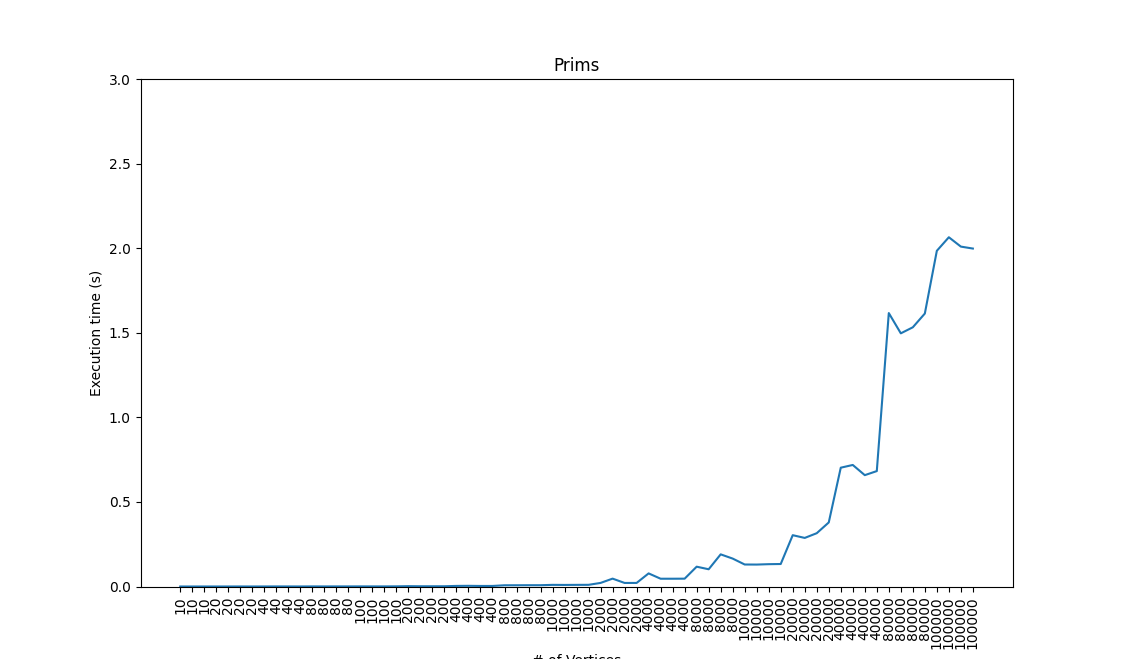
\includegraphics[width=19cm]{Img/Prims_Graph.png}
		\caption{Performance of Prim's Algorithm}
	\end{figure}

\pagebreak
\subsection{Graph of the performance of Kruskal's ''naive'' Algorithm}

	\begin{figure}[H]
		\hspace{-1cm}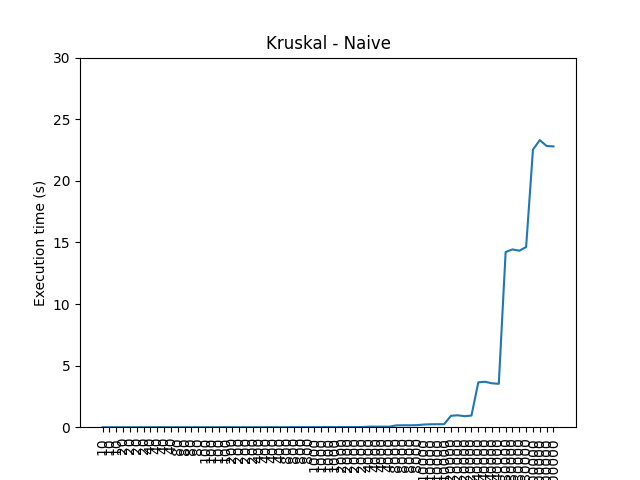
\includegraphics[width=19cm]{Img/Kruskal_Naive_Graph.png}
		\caption{Performance of Kruskal's ''naive'' Algorithm}
	\end{figure}

\pagebreak

\subsection{Graph of the performance of Kruskal's Union Find Algorithm}

	\begin{figure}[H]
		\hspace{-1cm}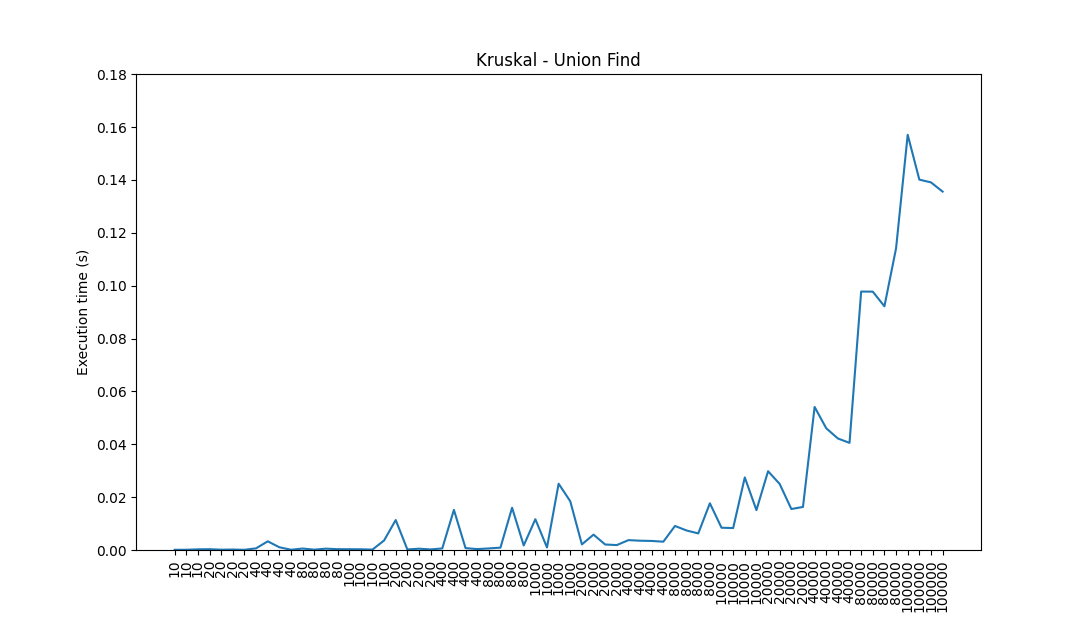
\includegraphics[width=19cm]{Img/Kruskal_UF_Graph.png}
		\caption{Performance of Kruskal's Union Find Algorithm}
	\end{figure}

\pagebreak